\documentclass[12pt]{extarticle}
\usepackage{tempora}
\usepackage[T1, T2A]{fontenc}
\usepackage[utf8]{inputenc}
\usepackage[english, ukrainian]{babel}
\usepackage{geometry}
\usepackage{graphicx}
\usepackage{multirow}
\usepackage{multicol}
\usepackage{float}
\graphicspath{{/home/artem/Pictures}}
\geometry
{
    a4paper,
    left=30mm,
    top=15mm,
    right=20mm,
    bottom=15mm,
}

\begin{document}
\begin{titlepage}
    \begin{center}
        \textbf{\normalsize{\MakeUppercase{
            Міністерство Освіти і науки України
            Національний університет "Львівська політехніка"
        }}}

        \begin{flushright}
        \textbf{ІКНІ}\\
        Кафедра \textbf{ПЗ}
        \end{flushright}
        \vspace{15mm}

        \includegraphics[width=0.4\textwidth]{lpnu_logo.png}

        \vspace*{\fill}

        \textbf{\normalsize{\MakeUppercase{Звіт}}}
            
        До лабораторної роботи №11

        \textbf{на тему:} “Метод пошуку Кнута-Мориса-Прата”

        \textbf{з дисципліни:} "Алгоритми і структури даних”
            
        \vspace*{\fill}

        \begin{flushright}

            \textbf{Лектор:}\\
            доцент кафедри ПЗ\\
            Коротєєва Т. О.\\
            \vspace{12pt}

            \textbf{Виконав:}\\
            студент групи ПЗ-24\\
            Губик А. С.\\
            \vspace{12pt}

            \textbf{Прийняв:}\\
            асистент кафедри ПЗ\\
            Вишневський К. О.\\
        \vspace{12pt}
        \end{flushright}

        Львів -- 2023
            
            
    \end{center}
\end{titlepage}

\subsection*{Тема роботи} 
Метод пошуку Бойера-Мура.
\subsection*{Мета роботи}  Вивчити алгоритм пошуку Бойера-Мура. Здійснити програмну реалізацію алгоритму пошуку Бойера-Мура.

 
\subsection*{Індивідуальне завдання}
Варіант 4.

Задано два тексти. В першому тексті знайти слово, що стоїть посередині тексту, замінити в ньому літери «а» на «о», «і» на «е» і знайти його входження в другий текст відповідним алгоритмом пошуку.

\subsection*{Теоретичні відомості}
Алгоритм Бойера-Мура базується на наступній схемі: порівняння символів починається з кінця слова. Нехай для кожного символу x слова dx - відстань від самого правого у слові входження х до кінця слова. Припустимо, знайдено неспівпадіння між словом та текстом на символі х в тексті. Тоді слово можна посунути вправо на dx позицій що є більше або рівне 1.

В даному алгоритмі символ х розглядається як стоп-символ - це є символ в тексті, який є першим неспівпадінням тексту і слова при порівнянні справа (з кінця слова). Розглянемо три можливих ситуації:

1)    Стоп-символ у слові взагалі не зустрічається, тоді зсув дорівнює довжині слова m.

2)    Крайня права позиція k входження стоп-символа у слові є меншою від його позиції j у тексті. Тоді слово можна зсунути вправо на k-j позицій так, щоб стоп-символ у слові і тексті опинились один під одним.

3)    Крайня права позиція k входження стоп-символа у слові є більшою від його позиції j у тексті. Тоді зсув дорівнює 1.

 

В найгіршому випадку алгоритм Бойера-Мура потребує n порівнянь, де n - кількість символів у тексті. У найкращих обставинах, коли останній символ слова завжди не співпадає з символом тексту, число порівнянь дорівнює n / m, де m - кількість символів слова. Отже складність алгоритму Бойера-Мура О(n / m).
\subsection*{Алгоритм}

Спочатку ми шукаємо символи які не є літерою, ми так повторюємо n / 2
разів, де n -- довжина тексту. Останній знайдений символ буде початком для
нової ітерації, в якій ми міняємо потрібні нам літери.

Алгоритм BM

Дано S[1…n] – стрічка, в якій відбувається пошук; P[1…m] – стрічка, входження якої у S необхідно найти;  i – індекс по S; j – індекс по P; stopChar – стопсимвол; answer – масив входжень стрічки P у S.

BM1.Присвоїти i = m. 

BM2.Повторювати кроки BM3-BM8 поки i<n.

BM3.Присвоїти i1=i. Якщо Si1 дорівнює Pj, то присвоїти j=j-1, i1=i1-1. 

BM4.Якщо j=0, то додати i-m до масиву answer. Присвоїти j=m. Перейти на крок 3.

BM5.Інакше присвоїти stopChar=Si1.

BM6.Якщо stopChar не зустрічається в P, то присвоїти i=i+m. Перехід на крок 3.

BM7.Якщо stopChar зустрічається в P, і позиція його входження в P(j1) є меншою за позицію в S(i1), то присвоїти i=i+(i1-j1). Перейти на крок 3.

BM8.Якщо stopChar зустрічається в P, і позиція його входження в P(j1) є більшою за позицію в S(i1), то присвоїти i=i+1. Перейти на крок 3.

BM9.Кінець. Вихід.

Складність алгоритму становить O(mn) в найгіршому випадку, О(n) в середньому
\subsection*{Вихідний код}

{\fontfamily{pcr}\selectfont
\begin{verbatim}
    #include <iostream>
    #include <fstream>
    #include <vector>
    #include <string>
    
    std::vector<int> computeLPS(const std::string& pattern) {
        int patternLength = pattern.length();
        std::vector<int> lps(patternLength, 0);
        int j = 0; // Length of the previous longest prefix suffix
    
        for (int i = 1; i < patternLength; ++i) {
            while (j > 0 && pattern[i] != pattern[j]) {
                j = lps[j - 1];
            }
    
            if (pattern[i] == pattern[j]) {
                lps[i] = ++j;
            }
        }
        return lps;
    }
    
    int findFirstOccurrence(const std::string& text, const std::string& pattern) {
        int textLength = text.length();
        int patternLength = pattern.length();
        std::vector<int> lps = computeLPS(pattern);
        for(int i : lps)
            std::cout << i << ' ';
        std::cout << std::endl;
        int j = 0; // Index for pattern[]
    
        for (int i = 0; i < textLength; ++i) {
            while (j > 0 && text[i] != pattern[j]) {
                j = lps[j - 1];
            }
    
            if (text[i] == pattern[j]) {
                if (j == patternLength - 1) {
                    return i - j; // Return the start index of the first occurrence
                } else {
                    j++;
                }
            }
        }
        return -1; // Pattern not found in text
    }
    
    int main() {
        std::ifstream file("input.txt"); // Replace "input.txt" with your file name
        if (!file.is_open()) {
            std::cout << "Unable to open file!" << std::endl;
            return 1;
        }
    
        std::string S, P;
        if (std::getline(file, S) && std::getline(file, P)) {
            int index = findFirstOccurrence(S, P);
            if (index != -1) {
                std::cout << "Pattern P found at index: " << index << std::endl;
            } else {
                std::cout << "Pattern P not found in string S" << std::endl;
            }
        } else {
            std::cout << "File does not contain both strings!" << std::endl;
        }
    
        file.close();
        return 0;
    }
    
\end{verbatim}
}

\vspace{12pt}
\begin{figure}[H]
    \centering
    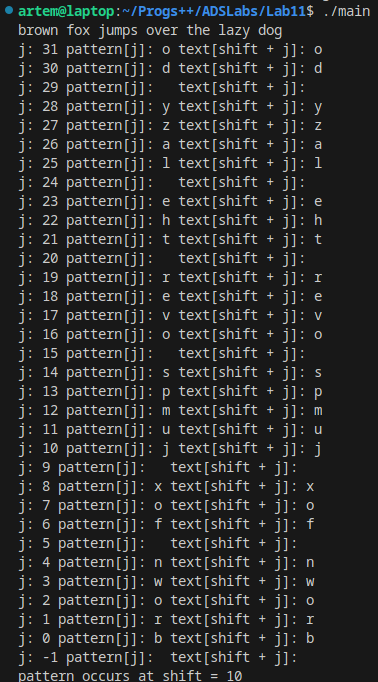
\includegraphics[width=0.90\textwidth]{Screenshot_20231206_085654}
    \caption{}
\end{figure}

\subsection*{Висновок} 

Я ознайомився з алгоритмом Кнута-Моріса-Прата і що таке Longest Suffix Prefix.

\end{document}
